\begin{figure}[h!]
    \centering
    \caption{Mean of all dependent variables for each season}
    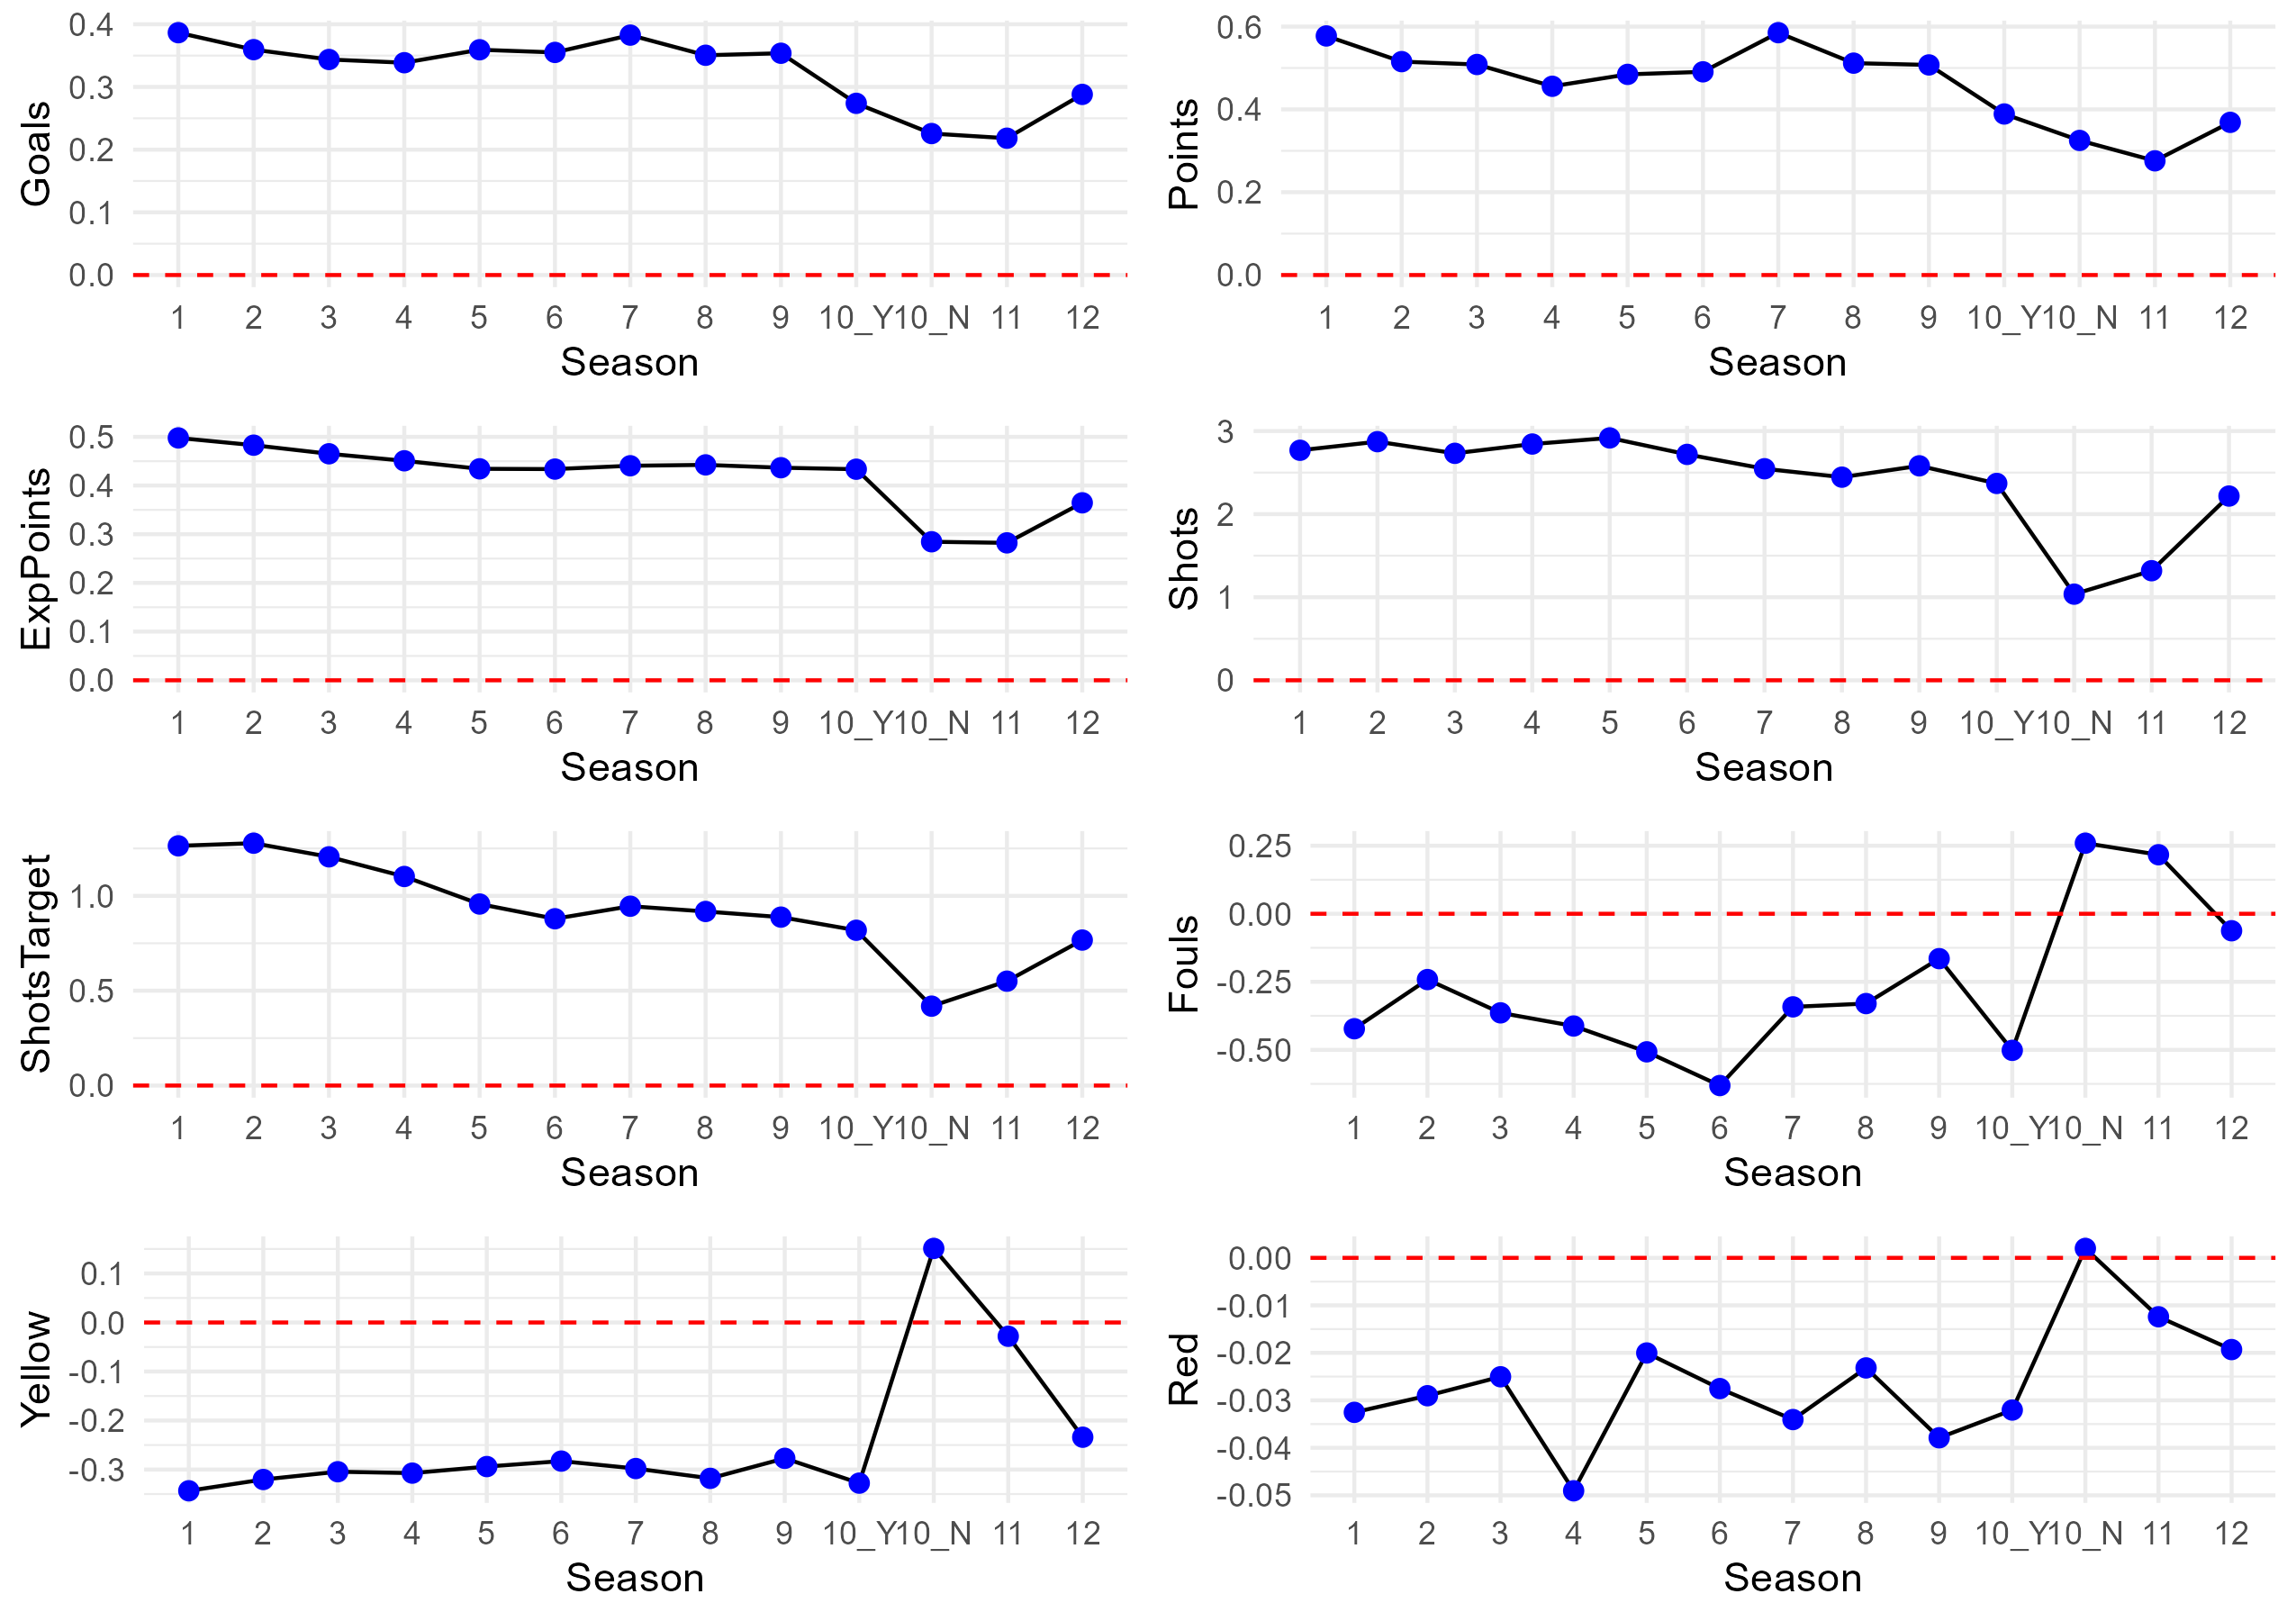
\includegraphics[width=1\textwidth]{Figures/Extended_plot.png}
    \label{fig:extend}
\end{figure}

\newpage

% NOTE
% FOR READABILITY I LET ALL TABLES HAVE A WIDER WIDTH THAN THE TEXT
% I at least limit it to be on both sides of the page

\begin{table}[H] \centering 
  \caption{Replication results over ten seasons for all dependent variables} 
  \label{tab:replic} 
  \addtolength{\leftskip} {-2cm}
  \addtolength{\rightskip}{-2cm}
\begin{tabular}{@{\extracolsep{5pt}}lD{.}{.}{-3} D{.}{.}{-3} D{.}{.}{-3} D{.}{.}{-3} } 
\\[-1.8ex]\hline 
\hline \\[-1.8ex] 
\\Difference H/A & \multicolumn{1}{c}{Goals} & \multicolumn{1}{c}{Points} & \multicolumn{1}{c}{Expected points} & \multicolumn{1}{c}{Shots} \\ 
\\[-1.8ex] & \multicolumn{1}{c}{(1)} & \multicolumn{1}{c}{(2)} & \multicolumn{1}{c}{(3)} & \multicolumn{1}{c}{(4)}\\ 
\hline \\[-1.8ex] 
  SpectatorsYes & 0.108 & 0.152 & 0.140^{***} & 1.406^{***} \\ 
  & (0.056) & (0.083) & (0.028) & (0.251) \\ 
  & & & & \\ 
 Season & -0.004 & -0.007 & -0.006^{***} & -0.045^{*} \\ 
  & (0.003) & (0.005) & (0.002) & (0.017) \\ 
  & & & & \\ 
 Constant & 0.224^{***} & 0.322^{***} & 0.280^{***} & 1.034^{***} \\ 
  & (0.055) & (0.081) & (0.029) & (0.243) \\ 
  & & & & \\ 
\hline \\[-1.8ex] 
$\sigma^2_{u}$ & \multicolumn{1}{c}{0.00} & \multicolumn{1}{c}{0.00} & \multicolumn{1}{c}{0.00} & \multicolumn{1}{c}{0.02} \\ 
$\sigma^2_{e}$ & \multicolumn{1}{c}{2.90} & \multicolumn{1}{c}{6.33} & \multicolumn{1}{c}{0.70} & \multicolumn{1}{c}{56.65} \\ 
Observations & \multicolumn{1}{c}{37,888} & \multicolumn{1}{c}{37,888} & \multicolumn{1}{c}{37,888} & \multicolumn{1}{c}{25,270} \\ 
Akaike Inf. Crit. & \multicolumn{1}{c}{147,903.700} & \multicolumn{1}{c}{177,432.700} & \multicolumn{1}{c}{94,139.760} & \multicolumn{1}{c}{173,741.500} \\ 
Bayesian Inf. Crit. & \multicolumn{1}{c}{147,946.400} & \multicolumn{1}{c}{177,475.500} & \multicolumn{1}{c}{94,182.470} & \multicolumn{1}{c}{173,782.200} \\ 
\hline 
\\Difference H/A & \multicolumn{1}{c}{Shots Target} & \multicolumn{1}{c}{Fouls} & \multicolumn{1}{c}{Yellow Cards} & \multicolumn{1}{c}{Red Cards} \\ 
\\[-1.8ex] & \multicolumn{1}{c}{(5)} & \multicolumn{1}{c}{(6)} & \multicolumn{1}{c}{(7)} & \multicolumn{1}{c}{(8)}\\ 
\hline \\[-1.8ex] 
 SpectatorsYes & 0.384^{**} & -0.589^{***} & -0.447^{***} & -0.033^{*} \\ 
  & (0.123) & (0.177) & (0.057) & (0.015) \\ 
  & & & & \\ 
 Season & -0.051^{***} & -0.009 & 0.003 & -0.0001 \\ 
  & (0.008) & (0.013) & (0.004) & (0.001) \\ 
  & & & & \\ 
 Constant & 0.418^{***} & 0.251 & 0.151^{**} & 0.002 \\ 
  & (0.118) & (0.198) & (0.055) & (0.014) \\ 
  & & & & \\ 
\hline \\[-1.8ex] 
$\sigma^2_{u}$ & \multicolumn{1}{c}{0.00} & \multicolumn{1}{c}{0.11} & \multicolumn{1}{c}{0.00} & \multicolumn{1}{c}{0.00} \\ 
$\sigma^2_{e}$ & \multicolumn{1}{c}{13.62} & \multicolumn{1}{c}{28.31} & \multicolumn{1}{c}{2.94} & \multicolumn{1}{c}{0.20} \\ 
Observations & \multicolumn{1}{c}{25,270} & \multicolumn{1}{c}{25,270} & \multicolumn{1}{c}{25,270} & \multicolumn{1}{c}{25,270} \\ 
Akaike Inf. Crit. & \multicolumn{1}{c}{137,729.600} & \multicolumn{1}{c}{156,230.800} & \multicolumn{1}{c}{98,962.080} & \multicolumn{1}{c}{31,171.130} \\ 
Bayesian Inf. Crit. & \multicolumn{1}{c}{137,770.300} & \multicolumn{1}{c}{156,271.500} & \multicolumn{1}{c}{99,002.770} & \multicolumn{1}{c}{31,211.810} \\ 
\hline 
\hline \\[-1.8ex] 
\textit{Note:}  & \multicolumn{4}{r}{$^{*}$p$<$0.05; $^{**}$p$<$0.01; $^{***}$p$<$0.001;} \\
& \multicolumn{4}{r}{$\sigma^2_{e}$ = Variance of first level residual error;}
& \multicolumn{5}{r}{$\sigma^2_{u}$ = Variance of second level residual error}
\end{tabular} 
\end{table} 

\begin{table}[H] \centering 
  \caption{Extended results over twelve seasons for all dependent variables}
  \label{tab:extend}
  \addtolength{\leftskip} {-2cm}
  \addtolength{\rightskip}{-2cm}
\begin{tabular}{@{\extracolsep{5pt}}lD{.}{.}{-3} D{.}{.}{-3} D{.}{.}{-3} D{.}{.}{-3} } 
\\[-1.8ex]\hline 
\hline \\[-1.8ex] 
\\ Difference H/A & \multicolumn{1}{c}{Goals} & \multicolumn{1}{c}{Points} & \multicolumn{1}{c}{Expected points} & \multicolumn{1}{c}{Shots} \\ 
\\[-1.8ex] & \multicolumn{1}{c}{(1)} & \multicolumn{1}{c}{(2)} & \multicolumn{1}{c}{(3)} & \multicolumn{1}{c}{(4)}\\ 
\hline \\[-1.8ex] 
 SpectatorsYes & 0.092^{**} & 0.145^{***} & 0.105^{***} & 0.996^{***} \\ 
  & (0.028) & (0.042) & (0.012) & (0.125) \\ 
  & & & & \\ 
 Season & -0.012^{***} & -0.019^{***} & -0.012^{***} & -0.084^{***} \\ 
  & (0.003) & (0.004) & (0.001) & (0.015) \\ 
  & & & & \\ 
 Constant & 0.061 & 0.071 & 0.125^{**} & 0.625^{**} \\ 
  & (0.044) & (0.064) & (0.048) & (0.199) \\ 
  & & & & \\ 
\hline \\[-1.8ex] 
$\sigma^2_{\upsilon}$ & \multicolumn{1}{c}{0.25} & \multicolumn{1}{c}{0.39} & \multicolumn{1}{c}{0.25} & \multicolumn{1}{c}{6.37} \\ 
$\sigma^2_{u}$ & \multicolumn{1}{c}{0.01} & \multicolumn{1}{c}{0.02} & \multicolumn{1}{c}{0.02} & \multicolumn{1}{c}{0.09} \\
$\sigma^2_{e}$ & \multicolumn{1}{c}{2.67} & \multicolumn{1}{c}{5.98} & \multicolumn{1}{c}{0.44} & \multicolumn{1}{c}{50.05} \\
Observations & \multicolumn{1}{c}{45,592} & \multicolumn{1}{c}{45,592} & \multicolumn{1}{c}{45,589} & \multicolumn{1}{c}{32,973} \\ 
Akaike Inf. Crit. & \multicolumn{1}{c}{175,114.400} & \multicolumn{1}{c}{211,776.900} & \multicolumn{1}{c}{94,092.890} & \multicolumn{1}{c}{223,438.800} \\ 
Bayesian Inf. Crit. & \multicolumn{1}{c}{175,166.800} & \multicolumn{1}{c}{211,829.300} & \multicolumn{1}{c}{94,145.260} & \multicolumn{1}{c}{223,489.300} \\ 
\hline 
\\Difference H/A & \multicolumn{1}{c}{Shots Target} & \multicolumn{1}{c}{Fouls} & \multicolumn{1}{c}{Yellow Cards} & \multicolumn{1}{c}{Red Cards} \\ 
\\[-1.8ex] & \multicolumn{1}{c}{(5)} & \multicolumn{1}{c}{(6)} & \multicolumn{1}{c}{(7)} & \multicolumn{1}{c}{(8)}\\ 
\hline \\[-1.8ex] 
 SpectatorsYes & 0.245^{***} & -0.402^{***} & -0.279^{***} & -0.018^{*} \\ 
  & (0.061) & (0.091) & (0.030) & (0.008) \\ 
  & & & & \\ 
 Season & -0.063^{***} & 0.028^{**} & 0.007 & 0.001 \\ 
  & (0.007) & (0.011) & (0.003) & (0.001) \\ 
  & & & & \\ 
 Constant & 0.145 & 0.255 & 0.041 & -0.008 \\ 
  & (0.101) & (0.136) & (0.032) & (0.007) \\ 
  & & & & \\ 
\hline \\[-1.8ex] 
$\sigma^2_{\upsilon}$ & \multicolumn{1}{c}{1.39} & \multicolumn{1}{c}{1.29} & \multicolumn{1}{c}{0.07} & \multicolumn{1}{c}{0.00} \\ 
$\sigma^2_{u}$ & \multicolumn{1}{c}{0.03} & \multicolumn{1}{c}{0.08} & \multicolumn{1}{c}{0.00} & \multicolumn{1}{c}{0.00} \\
$\sigma^2_{e}$ & \multicolumn{1}{c}{11.85} & \multicolumn{1}{c}{27.29} & \multicolumn{1}{c}{2.93} & \multicolumn{1}{c}{0.20} \\
Observations & \multicolumn{1}{c}{32,973} & \multicolumn{1}{c}{32,973} & \multicolumn{1}{c}{32,973} & \multicolumn{1}{c}{32,973} \\ 
Akaike Inf. Crit. & \multicolumn{1}{c}{175,913.300} & \multicolumn{1}{c}{203,158.900} & \multicolumn{1}{c}{129,429.800} & \multicolumn{1}{c}{40,881.940} \\ 
Bayesian Inf. Crit. & \multicolumn{1}{c}{175,963.700} & \multicolumn{1}{c}{203,209.300} & \multicolumn{1}{c}{129,480.200} & \multicolumn{1}{c}{40,932.360} \\ 
\hline 
\hline \\[-1.8ex] 
\textit{Note:}  & \multicolumn{4}{r}{$^{*}$p$<$0.05; $^{**}$p$<$0.01; $^{***}$p$<$0.001;} \\
& \multicolumn{4}{r}{$\sigma^2_{e}$ = Variance of first level residual error;}
& \multicolumn{5}{r}{$\sigma^2_{u}$ = Variance of second level residual error;}
& \multicolumn{5}{r}{$\sigma^2_{\upsilon}$ = Variance of third level residual error}
\end{tabular} 
\end{table} 

\begin{table}[H] \centering 
  \caption{Exploratory results over twelve Premier League seasons for all dependent variables}
  \label{tab:explor} 
  \addtolength{\leftskip} {-2cm}
  \addtolength{\rightskip}{-2cm}
\begin{tabular}{@{\extracolsep{5pt}}lD{.}{.}{-3} D{.}{.}{-3} D{.}{.}{-3} D{.}{.}{-3} } 
\\[-1.8ex]\hline 
\hline \\[-1.8ex] 
\\ Difference H/A & \multicolumn{1}{c}{Goals} & \multicolumn{1}{c}{Points} & \multicolumn{1}{c}{Expected points} & \multicolumn{1}{c}{Shots} \\ 
\\[-1.8ex] & \multicolumn{1}{c}{(1)} & \multicolumn{1}{c}{(2)} & \multicolumn{1}{c}{(3)} & \multicolumn{1}{c}{(4)}\\ 
\hline \\[-1.8ex] 
 Occupancy & 0.267^{**} & 0.447^{**} & 0.146^{**} & 1.500^{***} \\ 
  & (0.098) & (0.138) & (0.047) & (0.446) \\ 
  & & & & \\ 
 Season\_c & -0.021^{*} & -0.028^{*} & -0.022^{***} & -0.118^{**} \\ 
  & (0.009) & (0.013) & (0.004) & (0.042) \\ 
  & & & & \\ 
 Constant & -0.276^{*} & -0.419^{*} & -0.117 & -0.649 \\ 
  & (0.127) & (0.165) & (0.108) & (0.670) \\ 
  & & & & \\ 
\hline \\[-1.8ex] 
$\sigma^2_{u}$ & \multicolumn{1}{c}{0.34} & \multicolumn{1}{c}{0.50} & \multicolumn{1}{c}{0.38} & \multicolumn{1}{c}{11.32} \\ 
$\sigma^2_{e}$ & \multicolumn{1}{c}{3.01} & \multicolumn{1}{c}{6.01} & \multicolumn{1}{c}{0.68} & \multicolumn{1}{c}{62.53} \\ 
Observations & \multicolumn{1}{c}{4,558} & \multicolumn{1}{c}{4,558} & \multicolumn{1}{c}{4,558} & \multicolumn{1}{c}{4,558} \\ 
Log Likelihood & \multicolumn{1}{c}{-9,023.024} & \multicolumn{1}{c}{-10,594.960} & \multicolumn{1}{c}{-5,670.078} & \multicolumn{1}{c}{-15,947.010} \\ 
Akaike Inf. Crit. & \multicolumn{1}{c}{18,056.050} & \multicolumn{1}{c}{21,199.910} & \multicolumn{1}{c}{11,350.160} & \multicolumn{1}{c}{31,904.010} \\ 
Bayesian Inf. Crit. & \multicolumn{1}{c}{18,088.170} & \multicolumn{1}{c}{21,232.040} & \multicolumn{1}{c}{11,382.280} & \multicolumn{1}{c}{31,936.140} \\ 
\hline 
\\Difference H/A & \multicolumn{1}{c}{Shots Target} & \multicolumn{1}{c}{Fouls} & \multicolumn{1}{c}{Yellow Cards} & \multicolumn{1}{c}{Red Cards} \\ 
\\[-1.8ex] & \multicolumn{1}{c}{(5)} & \multicolumn{1}{c}{(6)} & \multicolumn{1}{c}{(7)} & \multicolumn{1}{c}{(8)}\\ 
\hline \\[-1.8ex] 
 Occupancy & 0.291 & -0.893^{***} & -0.101 & -0.014 \\ 
  & (0.219) & (0.256) & (0.087) & (0.020) \\ 
  & & & & \\ 
 Season\_c & -0.150^{***} & 0.005 & 0.029^{***} & 0.001 \\ 
  & (0.021) & (0.024) & (0.008) & (0.002) \\ 
  & & & & \\ 
 Constant & -0.798^{*} & 0.545^{*} & 0.072 & -0.004 \\ 
  & (0.336) & (0.272) & (0.085) & (0.017) \\ 
  & & & & \\ 
\hline \\[-1.8ex] 
$\sigma^2_{u}$ & \multicolumn{1}{c}{2.90} & \multicolumn{1}{c}{0.96} & \multicolumn{1}{c}{0.06} & \multicolumn{1}{c}{0.00} \\ 
$\sigma^2_{e}$ & \multicolumn{1}{c}{15.14} & \multicolumn{1}{c}{20.93} & \multicolumn{1}{c}{2.44} & \multicolumn{1}{c}{0.13} \\ 
Observations & \multicolumn{1}{c}{4,558} & \multicolumn{1}{c}{4,558} & \multicolumn{1}{c}{4,558} & \multicolumn{1}{c}{4,558} \\ 
Log Likelihood & \multicolumn{1}{c}{-12,715.650} & \multicolumn{1}{c}{-13,430.670} & \multicolumn{1}{c}{-8,527.484} & \multicolumn{1}{c}{-1,894.340} \\ 
Akaike Inf. Crit. & \multicolumn{1}{c}{25,441.290} & \multicolumn{1}{c}{26,871.350} & \multicolumn{1}{c}{17,064.970} & \multicolumn{1}{c}{3,798.679} \\ 
Bayesian Inf. Crit. & \multicolumn{1}{c}{25,473.410} & \multicolumn{1}{c}{26,903.470} & \multicolumn{1}{c}{17,097.090} & \multicolumn{1}{c}{3,830.803} \\   
\hline 
\hline \\[-1.8ex] 
\textit{Note:}  & \multicolumn{4}{r}{$^{*}$p$<$0.05; $^{**}$p$<$0.01; $^{***}$p$<$0.001;} \\
& \multicolumn{4}{r}{$\sigma^2_{e}$ = Variance of first level residual error;}
& \multicolumn{5}{r}{$\sigma^2_{u}$ = Variance of second level residual error}
\end{tabular} 
\end{table} 